%%=============================================================================
%% Proof of concept
%%=============================================================================

\chapter{\IfLanguageName{dutch}{Proof of concept}{Proof of concept}}%
\label{ch:proof of concept}

\section{\IfLanguageName{dutch}{De POC omgeving}
{The POC environment}}
\label{sec:De POC omgeving}

Aan de hand van deze POC wordt er onderzocht hoe veilig het is om secrets te gebruiken in Jenkins. De infrastructuur van deze POC is uitgerold in de cloud. De infrastructuur die gebruikt wordt, wordt automatisch gedeployed aan de hand van terraform. Deze infrastructuur wordt opgebouwd door gebruik te maken van de AWS provider voor terraform. De infrastructuur bestaat uit een bastion server, een Jenkins server, een AWS scaling group en een Kubernetes cluster. Deze componenten werken te samen en vormen de fictieve productie omgeving. Deze infrastructuur laat toe een applicatie te bouwen aan de hand van een CI/CD pipeline. Op het CI gedeelte van deze pipeline worden enkele aanvallen uitgevoerd om secrets te extraheren uit de omgeving en te onderzoeken hoe deze aanvallen vermeden kunnen worden. Binnen dit gedeelte worden ook enkele concepten uit de DevSecOps toegepast om een veilige pipeline te creeëren.

\begin{itemize}
  \item De container wordt gescanned in de CD pipeline voor vulnerabilities.
  \item Er wordt gebruik gemaakt van een secret store om credentials op te slaan.
  \item Secrets worden geïncrypteerd in de deployment pipeline.
\end{itemize}

Het CD gedeelte volgt de GitOps aanpak en de secrets die gebruikt worden binnen de pipeline worden geïncrypteerd.

\subsection{\IfLanguageName{dutch}{Prerequisites}
{Prerequisites}}
\label{sec:Prerequisites}

Om deze omgeving op te bouwen wordt er gebruik gemaakt van enkele belangrijke software. Deze sofware wordt geïnstalleerd en aan PATH toegevoegd zodat deze eenvoudig gebruikt kan worden vanaf de commandline.

\begin{itemize}
  \item Het uitrollen van de omgeving is volledig geautomatiseerd met Terraform.
  \item Om AWS vanaf de commandline te gebruiken wordt aws cli gebruikt.
  \item Om kubernetes vanaf de commandline te gebruiken wordt kubectl gebruikt.
  \item Om de Java app te bouwen en te testen wordt maven gebruikt.
  \item Om de docker container te testen wordt docker desktop gebruikt.
\end{itemize}

Aangezien er bij het CD gedeelte van de pipeline gebruik wordt gemaakt van secrets, wordt de Sealed secrets extensie voor vscode ook geïnstalleerd.

\subsubsection{\IfLanguageName{dutch}{Bouwen en testen van de applicatie}
{Building and testing the application}}
\label{sec:Bouwen en testen van de applicatie}

Om uiteindelijk het bouwproces van een applicatie te simuleren wordt een test java applicatie gebouwd. Deze applicatie toont om de 5 seconden het bericht "hello world". Deze functionaliteit is nodig omdat deze applicatie moet draaien op een kubernetes cluster. Op die manier kan een service gesimuleerd worden die in een docker container uitgevoerd kan worden. De code snippit voor de java app kan hieronder teruggevonden worden.
\newline

\begin{lstlisting}
package vvanhooren;

  /**
   * Hello world!
   *
   */
  public class App 
  {
      public static void main( String[] args )
      {
          while(true) {
              System.out.println("hello world");
              try {
                  Thread.sleep(5000); // wait for 5 seconds
              } catch (InterruptedException e) {
                  e.printStackTrace();
              }
          }
      }
  }
\end{lstlisting}
\vspace{4cm}
Na het bouwen van de applicatie wordt getest of deze correct gecompileer kan worden met maven. Om deze applicatie uiteindelijk te kunnen gebruiken in een deployment omgeving, wordt een docker image gemaakt. Deze eenvoudige docker image maakt gebruik van een bestaande image waar maven en java op geinstalleerd zijn. In deze image wordt een copy uitgevoerd om de gecompileerde applicatie te kopieren naar de nieuwe docker image en de applicatie wordt uitgevoerd door een java commando te runnen. Door gebruik te maken van Docker desktop kan getest worden of de container stabiel is. De code voor de dockerimage kan hieronder teruggevonden worden.
\newline

\begin{lstlisting}[style=dockerfile,language=Dockerfile]
  # Use official Maven image with Alpine base image
  FROM maven:3.9-ibmjava AS build
  
  # Copy the jar file 
  COPY ./target/*.jar /app/app.jar
  
  # Set the working directory in the container
  WORKDIR /app
  
  # Run the app
  CMD ["java","-jar","app.jar"]
\end{lstlisting}

\subsubsection{\IfLanguageName{dutch}{Bouwen van de Kubernetes deployment}
{Building the Kubernetes deployment}}
\label{sec:Bouwen van de Kubernetes deployment}

De applicatie zal uiteindelijk worden uitegerold op een kubernetes cluster die in AWS draait. Omdat er gebruikt wordt gemaakt van Kustomize om de kubernetes manifest bestanden te beheren,wordt de bestandenstructuur in figuur \ref{fig:bestandstructuur} gebruikt.
\newline

\begin{figure}[H]
    \dirtree{%
    .1 myargo-app/.
    .2 README.md.
    .2 environments/.
    .3 staging/.
    .4 my-app/.
    .5 kustomization.yaml.
    .2 my-app-base/.
    .3 deployment.yaml.
    .3 kustomization.yaml.
    .3 namespace.yaml.
    }
  \caption{\label{fig:bestandstructuur}bestandstructuur voor de staging omgeving}
\end{figure}
\vspace{4cm}
Deze repostiory is voorzien van een kubernetes deployment object zodat de container met de java applicatie uit de vorige stap correct uitgerold kan worden. Daarnaast wordt een namespace kubernetes object voorzien. Er wordt gebruik gemaakt van Kustomization files om de kubernetes configuratie beter te kunnen beheren. Op die manier wordt de applicatie code gescheiden van de configuratie code en wordt er overzicht bewaard binnen de gehele repository.
\newline

De deployment object bestaat uit een container die op poort 80 draait. De image wordt opgehaald van de private docker repository die gebruikt zal worden in de CI pipeline. Onderstaande code toont hoe dit kubernetes object wordt geconfigureerd. 
\newline

\begin{lstlisting}[style=kubernetesyaml,language=kubernetesyaml]
  ---
  apiVersion: apps/v1
  kind: Deployment
  metadata:
    name: my-maven-app
    labels:
      app: maven-app
  spec:
    selector:
      matchLabels:
        app: maven-app
    template:
      metadata:
        labels:
          app: maven-app
      spec:
        containers:
          - name: maven-app
            imagePullPolicy: Always
            image: victorwillem/my_maven_app
            ports:
              - containerPort: 90
\end{lstlisting}

\vspace{0.5cm}
Het kubernetes namespace object definieert een nieuwe namespace waar de pod zal runnen. De volgende code toont hoe deze yaml file is opgebouwd.
\newline

\begin{lstlisting}[style=kubernetesyaml,language=kubernetesyaml]
  ---
  apiVersion: v1
  kind: Namespace
  metadata:
    name: maven
\end{lstlisting}

\vspace{2cm}

Het kustomization bestand in de my-app-base folder wordt gebruikt om te bepalen welke bestanden overschreven kunnen worden. De deployment en namespace objecten worden overschreven binnen deze opstelling. Dit bestand is op deze manier opgebouwd.
\newline 

\begin{lstlisting}[style=kubernetesyaml,language=kubernetesyaml]
  ---
  apiVersion: kustomize.config.k8s.io/v1beta1
  kind: Kustomization
  metadata:
    name: arbitrary
  resources:
    - deployment.yaml
    - namespace.yaml 
\end{lstlisting}

\vspace{0.5cm}
Tenslotte wordt nog een kustomize file voorzien in de staging omgeving. Dit configuratie bestand bepaalt hoeveel replicas (pods) er uiteindelijk op de cluster zullen runnen en eventuele configuratie elementen van de kubernetes files die overschreven zullen worden. Ook bevat dit bestand andere configuratie elementen zoals de locatie van de kubernetes secret die gebruikt wordt voor de private docker repository.
\newline

\begin{lstlisting}[style=kubernetesyaml,language=kubernetesyaml]
  ---
  namespace: staging
  replicas:
    - name: my-maven-app
      count: 1
  images:
    - name: victorwillem/my_maven_app
      newTag: v0.1.0
  resources:
    - "../../../my-app-base"
  patches:
    - target:
        kind: Deployment
      patch: |-
        - op: add
          path: /spec/template/spec/imagePullSecrets
          value: [{ name: dockerconfigjson }]
\end{lstlisting}

\vspace{0.5cm}
Indien er andere omgevingen worden opgezet zoals een productie omgeving, moet een nieuwe bestanden structuur opgebouwd worden met een nieuw kustomization bestand. Deze wordt duidelijk in figuur \ref{fig:bestandstructuurnieuw}

\begin{figure}[H]
  \dirtree{%
  .1 myargo-app/.
  .2 README.md.
  .2 environments/.
  .3 staging/.
  .4 my-app/.
  .5 kustomization.yaml.
  .3 production/.
  .4 my-app/.
  .5 kustomization.yaml
  .2 my-app-base/.
  .3 deployment.yaml.
  .3 kustomization.yaml.
  .3 namespace.yaml.
  }
\caption{\label{fig:bestandstructuurnieuw}bestandstructuur voor productie en staging omgeving}
\end{figure}

\subsubsection{\IfLanguageName{dutch}{Terraform backend configuratie}
{Terraform backend configuration}}
\label{sec:Terraform backend configuratie}

Vooraleer de infrastructuure en het netwerk opgebouwd kan worden met terraform, is het belangrijk de terraform tfstate bestand te bewaren op een veilig plek. Bij deze POC opstelling wordt gebruik gemaakt van een AWS S3 bucket om dit bestand op een veilige plek te bewaren. Om te voorkomen dat meerdere instanties hetzelfde state bestand aanpassen maakt terraform gebruik van de state lock. Door dit bestand ook ergens te bewaren kunnen meerdere mensen gebruik maken van dezelfde terraform configuratie. Dit bestand wordt in deze POC bewaard door gebruik te maken van de AWS dynamo db. Dit kan aan de hand van terraform of handmatig de terraform configuratie voor deze componenten kan hieronder teruggevonden worden.
\newline

\begin{lstlisting}[language=terraform]
  resource "aws_s3_bucket" "terraform_state_environment" { 
    bucket = "terraform-state-environment-victorwillem" 
      
      lifecycle { 
        prevent_destroy = true 
    } 
  }

  resource "aws_s3_bucket_versioning" "versioning_s3" {
    bucket = aws_s3_bucket.terraform_state_environment.id
    versioning_configuration {
      status = "Enabled"
    }
  }
  
  resource "aws_s3_bucket_server_side_encryption_configuration" "encryption_s3" {
      bucket = aws_s3_bucket.terraform_state_environment.id
      rule {
        apply_server_side_encryption_by_default {
          sse_algorithm = "AES256"
        }
      }
    
  }

  resource "aws_dynamodb_table" "forcestate" {
    name = "for_state_lock"
    hash_key = "LockID"
    read_capacity = "8"
    write_capacity = "8"

    attribute {
      name = "LockID"
      type = "S"
    }
    tags = {
        Name = "StateLock"
    }
  
}
\end{lstlisting}

\subsubsection{\IfLanguageName{dutch}{Netwerkconfiguratie en beveiliging met AWS security groups}
{Networkconfiguration and security with AWS security groups}}
\label{sec:Netwerkconfiguratie en beveiliging met AWS security groups}

\paragraph{\IfLanguageName{dutch}{Netwerkarchitectuur overzicht}
{Overview of the network architecture}}
\label{sec:Netwerkarchitectuur overzicht}

Het netwerk is volledig opgebouwd met terraform. Het netwerk bestaat uit een virtual private network (VPC) die geconecteerd is met verschillende subnets. Deze subnets zijn verspreid over verschillende availability zones. Er zijn drie private subnets voorzien en drie publieke subnets. Twee subnets van elke categorie zijn in gebruik voor de kubernetes cluster. In de documentatie van EKS het kubernetes product op AWS wordt aangeraden om zoveel subnets te voorzien zodat er voldoende redundantie is binnen de opstelling. Het laatste private subnet is gereserveerd voor de jenkins server, AWS scaling groep en andere servers die opgebouwd worden om de aanvallen te testen. Het laatste publieke subnet is gereserveerd voor de bastion server. Er is slechts één internet gateway voorzien die verbonden is met alle publieke subnets, de private subnets kunnen aan het internet via verschillende NAT gateways. 
\newline

Om deze connecties mogelijk te maken zijn er verschillende route tabellen geconfigureerd. De subnets van de kubernetes cluster zijn voorzien van speciale tags zodat interne of externe load balancers geconfigureerd kunnen worden. In deze configuratie wordt geen gebruik gemaakt van deze load balancers voor de kubernetes opstelling. Er wordt wel gebruik gemaakt van publieke loadbalancers om jenkins en sonarqube te exposen naar het internet toe.
\clearpage

De volledige netwerk configuratie wordt duidelijk weergegeven aan de hand van figuur \ref{fig:aws_network} en figuur \ref{fig:aws_networkfigure}

\begin{figure}[H]
  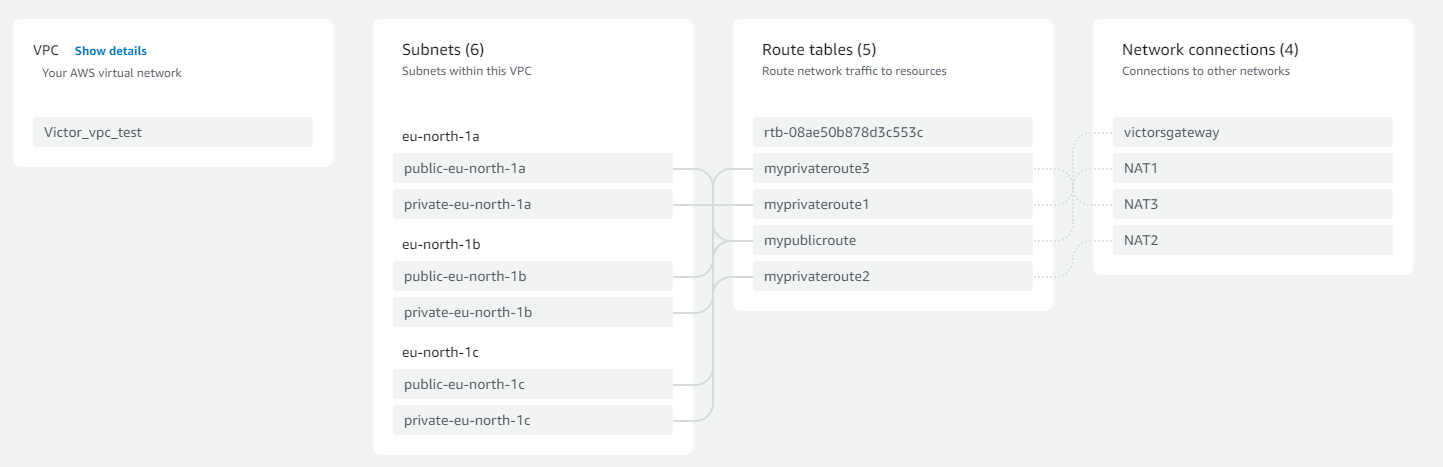
\includegraphics[scale=0.48]{graphics/aws_network.png}
\caption{\label{fig:aws_network} globaal overzicht van het netwerk}
\end{figure}

\begin{figure}[H]
  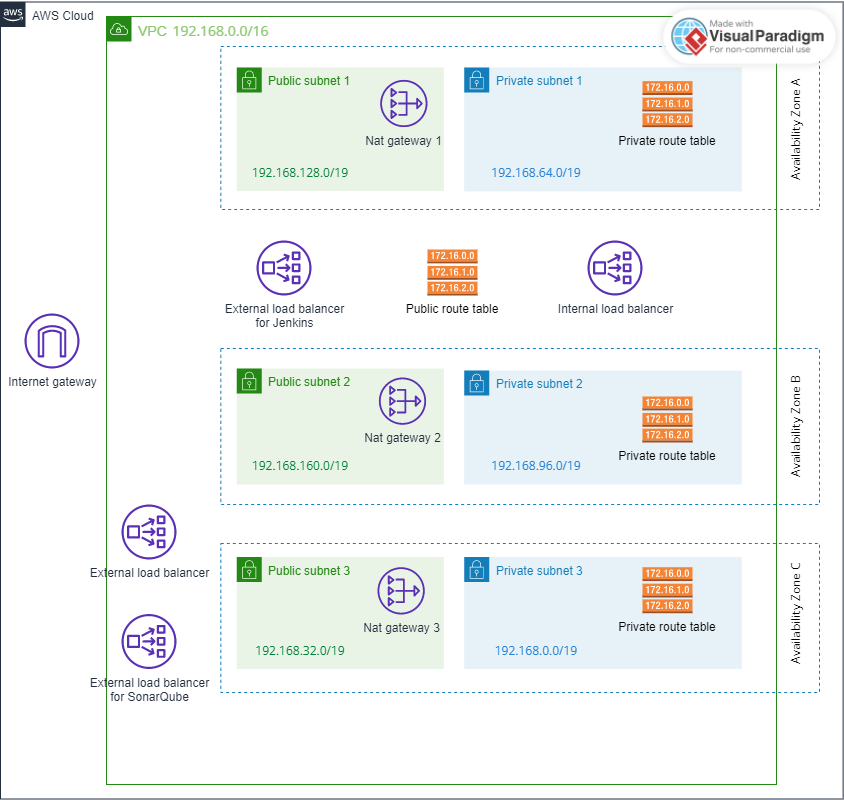
\includegraphics[scale=0.45]{graphics/network.png}
\caption{\label{fig:aws_networkfigure} het netwerk waarvan de POC opstelling gebruik maakt}
\end{figure}

\paragraph{\IfLanguageName{dutch}{Bouwen van het netwerk en de security groups met terraform}
{Building the network and the security groups using terraform}}
\label{sec:Bouwen van het netwerk en de security groups met terraform}

Om een omgeving in terraform op te stellen die hergebruikt kan worden, wordt bij elke component van het netwerk zoveel mogelijk met parameters gewerkt. De parameters worden ingesteld in het terraform tfvars bestand. Elke componente wordt ook waar mogelijk voorzien van een eigen module die ingeladen wordt in het main terraform bestand.
\newline

De VPC wordt op onderstaande manier opgebouwd. De id van de vpc die aangemaakt wordt, wordt gebruikt om andere componenten in het netwerk te configureren en wordt dus als een output voorzien binnen deze module.
\newline

\begin{lstlisting}[language=terraform]
  # Bouwen van een aws vpc component
  resource "aws_vpc" "main" {
  
    # Instellen van de vpc cidr block
    cidr_block = var.vpc_cidr
  
    # Instellen van de vpc naam
    tags = var.vpc_name
  
    # aanzetten van bepaalde dns instellingen die nodig zijn voor deze vpc
    enable_dns_hostnames = true
    enable_dns_support = true
  
  }
\end{lstlisting}

\vspace{0.5cm}
De subnets worden voorzien van ingress and egress regels zodat het netwerkverkeer gecontroleerd kan worden van en naar de verschillende netwerkcomponenten. Om deze regels te kunnen configureren moeten er eerst security groups aangemaakt worden. Deze security groups worden vervolgens gelinkt met toepasselijke regels. De security groups worden op deze manier geconfigureerd. Deze componten in de opstelling zijn afhankelijk van de VPC en gebruiken de output van de VPC module om correct ingesteld te worden.
\newline

\begin{lstlisting}[language=terraform]
  # Resource block die gebruikt wordt om een security group aan te maken
  resource "aws_security_group" "group1" { 
  
    # Instellen van de security group naam
    name   = var.aws_security_group
  
    # Instellen van de vpc id
    vpc_id = var.vpc_id 
  
    # Instellen van de security group tags
    tags = var.aws_security_group_name
  }
\end{lstlisting}

\vspace{0.5cm}
De verschillende ingress and egress regels worden geconfigureerd aan de hand van volgende terraform code. Afhankelijk van het soort regel worden enkele elementen toegevoegd bij de security group. Sommige regels worden niet geconfigureerd voor een bepaalde cidr, maar eerder voor een bepaalde security group. Daarnaast zijn sommige regels ook geconfigureerd om alle protcollen toe te laten. Welke instelling een regel krijgt hang af van hoe deze georienteerd staat, met andere woorden of het om een ingress of egress regel gaat. Bij deze modules wordt ook gebruik gemaakt van data sources en locals om alle parameters in te stellen.
\newline

De terraform configuratie voor een ingress rule met als bron een bepaalde security group ziet er zo uit.
\newline

\begin{lstlisting}[language=terraform]
  # Resource block die gebruikt wordt om een ingress rule in te stellen
  resource "aws_vpc_security_group_ingress_rule" "name" {
  
      # Instellen van het bereik (van poort ... tot poort ...)
      from_port = var.aws_security_group_from
      to_port = var.aws_security_group_to
  
      # Instellen van het protocol waarop deze security rule van toepassing is tcp/udp of -1 voor beide
      ip_protocol = var.aws_security_group_rule_protocol
  
      # Id van de security group die gebruikt zal worden als de source van het verkeer
      referenced_security_group_id = data.aws_security_group.source.id
  
      # Id van de security group zodat deze rule aan deze group gekoppeld kan worden
      security_group_id = data.aws_security_group.name.id
    
  }
\end{lstlisting}

\vspace{0.5cm}
De terraform configuratie voor een ingress rule met als bron een cidr wordt op deze manier geconfigureerd.
\newline

\begin{lstlisting}[language=terraform]
  # Resource block die gebruikt wordt om een ingress rule in te stellen
  resource "aws_vpc_security_group_ingress_rule" "name" {
  
      # de cidr die gebruikt zal worden als de source van het verkeer
      cidr_ipv4 = local.cidr_ipv4
  
      # Instellen van het bereik (van poort ... tot poort ...)
      from_port = var.aws_security_group_from
      to_port = var.aws_security_group_to
  
      # Instellen van het protocol waarop deze security rule van toepassing is tcp/udp of -1 voor beide
      ip_protocol = var.aws_security_group_rule_protocol
  
      # Id van de security group zodat deze rule aan deze group gekoppeld kan worden
      security_group_id = data.aws_security_group.name.id
    
  }
\end{lstlisting}

\vspace{0.5cm}
De terraform configuratie voor een egress rule met als bestemming een cidr ziet er zo uit.
\newline

\begin{lstlisting}[language=terraform]  
  # Resource block die gebruikt wordt om een ingress rule in te stellen
  resource "aws_vpc_security_group_egress_rule" "name" {
  
      # de cidr die gebruikt zal worden als de source van het verkeer
      cidr_ipv4 = local.cidr_ipv4
      
      # Instellen van het protocol waarop deze security rule van toepassing is tcp/udp of -1 voor beide
      ip_protocol = var.aws_security_group_rule_protocol
  
      # Id van de security group zodat deze rule aan deze group gekoppeld kan worden
      security_group_id = data.aws_security_group.name.id
    
  }
\end{lstlisting}

\vspace{0.5cm}
De VPC is gelinkt met alle subnets. Bij deze opstelling worden private en publieke subnets voorzien. Deze subnets zijn verspreid over meerder availability zones op die manier is er extra redundantie. De id's van de aangemaakte subnets worden gebruikt voor het maken van de servers en de cluster.
\newline

De configuratie om een private subnet in te stellen kan hieronder teruggevonden worden. Bij de configuratie van een publiek subnet wordt de parameter "map public ip on launch toegevoegd".
\newline
\begin{lstlisting}[language=terraform]  
  # Resource block die gebruikt wordt om een private subnet in te stellen
  resource "aws_subnet" "private_subnet" {
  
    # Instellen van de VPC id
    vpc_id     = var.vpc_id
  
    # Instellen van de cidr
    cidr_block = var.private_subnet_cidr
  
    # Instellen van de naam en andere tags
    tags       = var.private_subnet_tags
  
    # Instellen van de AWS availability zone
    availability_zone = var.private_subnet_availability_zone
  } 
\end{lstlisting}

\vspace{0.5cm}
De meeste basis componenten van het netwerk zijn op dit moment geconfigureerd, maar de toegang naar het internet ontbreekt nog, de gateways. De publieke subnets worden gelinkt aan één internet gateway en de private worden elk voorzien van een nat gateway. Op die manier kunnen instanties uit de verschillende subnets aan het internet indien dit een vereiste zou zijn.
\newline

De internet gateway wordt op deze manier geconfigureerd. De id van deze resource wordt gebruikt voor het configureren van de route tabellen.
\newline

\begin{lstlisting}[language=terraform]  
  # Resource block die gebruikt wordt om een internet gateway in te stellen
  resource "aws_internet_gateway" "name" {
  
      # Instellen van de VPC id
      vpc_id = var.vpc_id
  
      # Instellen van de internet gateway naam
      tags = var.aws_internet_gateway_name
  
    
  }
\end{lstlisting}

\vspace{0.5cm}
In een nat gateway worden de private ip-adressen vertaald naar publieke, daarom moeten er eerst nog elastic ip-adressen geconfigureerd worden in AWS. Elastic ip-adressen zorgen ervoor dat de nat gateways een publiek adres krijgen. De elastic ip-adressen worden op deze manier geconfigureerd.
\newline

\begin{lstlisting}[language=terraform]  
  # Resource block die gebruikt wordt om een elastic ip-adres in te stellen
  resource "aws_eip" "nat1" {
  
      # Instellen van de elastic ip adres naam
      tags = var.aws_eip_name 
  }
\end{lstlisting}

\vspace{0.5cm}
Om de nat gateways te configureren wordt deze terraform configuratie gebruikt. De output van deze component wordt opnieuw gebruikt bij het bouwen van de verschillende route tabellen.
\newline

\begin{lstlisting}[language=terraform]  
  # Resource block die gebruikt wordt om een nat gateway in te stellen
  resource "aws_nat_gateway" "example" {
  
    # Instellen van het elastic ip adres dat gekoppelt wordt aan deze resource
    allocation_id = var.aws_eip_id
  
    # Instellen van het publieke subnet dat gekoppelt wordt aan deze resource
    subnet_id     = var.public_subnet_id
  
    # Instellen van de nat gateway naam
    tags = var.aws_nat_gateway_name
  }
\end{lstlisting}

\vspace{0.5cm}
De laatste stap om het netwerk werkende te krijgen is het toevoegen van de routes. Alle componenten zijn ondertussen al opgebouwd, maar er is nog geen route tabel gebouwd die ervoor zorgt dat de resource het internet kunnen gebruiken. Om deze laatste stap van het netwerk correct te configureren wordt gebruik gemaakt van de "AWS route table" resource. 
\newline

Om een private route tabel te configureren wordt volgende code blok gebruikt. Bij een publieke route tabel wordt gebruik gemaakt van de nat gateway id in de plaats van de internet gateway id.
\newline

\begin{lstlisting}[language=terraform]  
  # Resource block die gebruikt wordt om een nat gateway in te stellen
  resource "aws_route_table" "route_table_private" {
  
      # Instellen van de VPC id
      vpc_id = var.aws_vpc_id
  
      # Instellen van de route
      route {
  
          # Instellen van de cidr
          cidr_block = var.aws_route_table_private_cidr
  
          # Instellen van de gateway die gebruikt zal worden
          gateway_id = var.aws_nat_gateway_id
      }
  
      # Instellen van de route tabel naam
      tags = var.aws_route_table_private_name
    
  }
\end{lstlisting}

\vspace{0.5cm}
De route tabellen moeten uiteindelijk nog gelinkt worden aan de correcte subnets. Via volgende code wordt deze link op de juiste manier opgebouwd.

\begin{lstlisting}[language=terraform]  
  # Resource block die gebruikt wordt om een route tabel link in te stellen
  resource "aws_route_table_association" "route_association_public" {
      
      # Instellen van het correcte subnet
      subnet_id = var.aws_subnet_public_id
  
      # Instellen van de route tabel die gebruikt zal worden
      route_table_id = var.aws_route_table_public_id
  }
  
\end{lstlisting}

% \paragraph{\IfLanguageName{dutch}{Infrastructuur overzicht}
% {Overview of the infrastructure}}
% \label{sec:Infrastructuur overzicht}

De infrastructuur wordt opgebouwd door gebruik te maken van terraform. In deze opstelling worden enkele servers voorzien. De jenkins server is verantwoordelijk voor alle bouwopdrachten. Deze server is het hart van de CD pipeline. De bouwopdrachten worden niet rechstreeks uitgevoerd op deze server, deze server stuurt een AWS autoscaling groep aan die nieuwe ec2 instances toevoegt wanneer nieuwe builds worden aangevraagd. Door gebruik te maken van een autoscaling groep is het mogelijk om deze instances ook af te breken wanneer deze niet meer nodig zijn. 
\newline

De bouwopdrachten worden dus uitgevoerd op aparte ec2 instances, genaamd jenkins runners. De jenkins runners en de jenkins master server maken beide gebruik van een baked image op die manier is er geen nood aan extra scripts wanneer de instance  opgestart wordt. Deze manier van werken laat ook toe om verschillende soorten jenkins runners te bouwen voor verschillende soorten pipelines. De configuratie van de jenkins server wordt voorzien aan de hand van een "jenkins as code". Deze configuratie file is opgeslagen in een aparte S3 bucket en wordt ingeladen bij het opstarten van de jenkins server.
\newline

Deze jenkins server is niet direct verbonden met het internet er is een loadbalancer voorzien om toegang te krijgen tot de login pagina. Deze server is ook enkel beschikbaar in een private subnet. Er wordt gebruik gemaakt van een nat gateway om internet te voorzien en via een bastion server is er een mogelijkheid om naar deze machine te sshen.
\newline

Verder is op deze server ook een sonarqube container aanwezig die sonarqube voorziet. Ook sonarqube is toegankelijk via een loadbalancer. De jenkinsserver beschikt daarnaast over enkele software die nodig is om correct te functioneren.
\newline


% \begin{figure}[H]
%   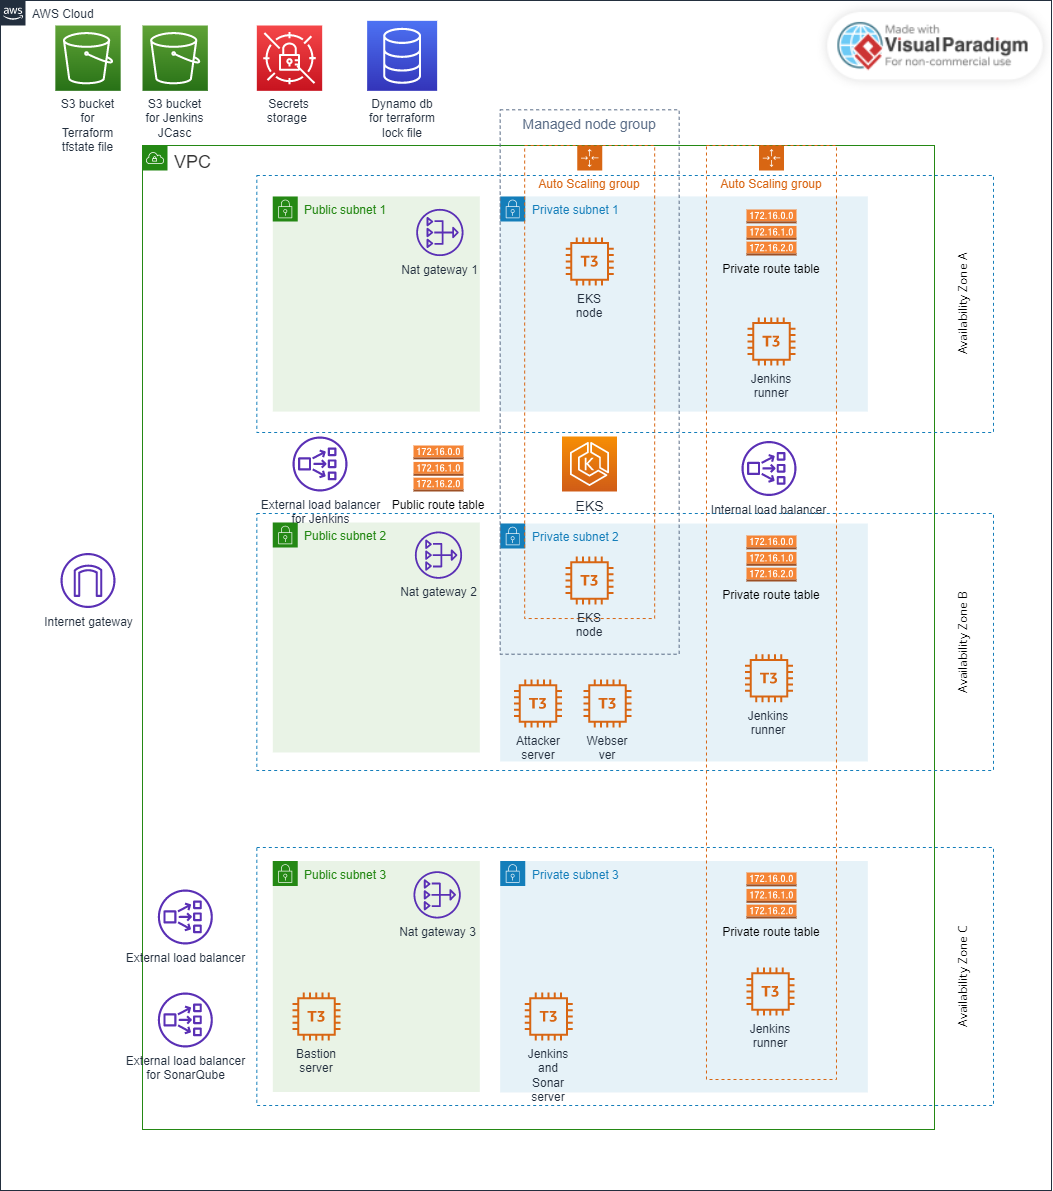
\includegraphics[scale=0.50]{graphics/infrastructuur.png}
% \caption{\label{fig:aws_infrastructuur} De infrastructuur waar de POC gebruik van maakt}
% \end{figure}

% \paragraph{\IfLanguageName{dutch}{Bouwen van de infrastructuur met terraform}
% {Building the infrastructure with terraform}}
% \label{sec:Bouwen van de infrastructuur met terraform}





























































\subsubsection{\IfLanguageName{dutch}{Post deployment}
{Post deployment}}
\label{sec:Post deployment}

\subsection{\IfLanguageName{dutch}{De CI/CD pipeline opzetten}
{Building the CI/CD pipeline}}
\label{sec:Bouwen van de CI/CD pipeline}

\subsubsection{\IfLanguageName{dutch}{Bouwen van de CI pipeline}
{Building the CI pipeline}}
\label{sec:Bouwen van de CI pipeline}

\subsubsection{\IfLanguageName{dutch}{Bouwen van de CD pipeline}
{Building the CI/CD pipeline}}
\label{sec:Bouwen van de CD pipeline}

\section{\IfLanguageName{dutch}{Aanvallen op de POC omgeving}
{Attacks on the POC environment}}
\label{sec:Aanvallen op de POC omgeving}

\subsection{\IfLanguageName{dutch}{Aanval 1}
{Aanval 1}}
\label{sec:Aanval 1}

\subsubsection{\IfLanguageName{dutch}{Aanval scenario}
{Attack scenario}}
\label{sec:Aanval scenario}

\subsubsection{\IfLanguageName{dutch}{Impact}
{Impact}}
\label{sec:Impact}

\subsubsection{\IfLanguageName{dutch}{Aanbevelingen}
{Recommendations}}
\label{sec:Aanbevelingen}

\subsection{\IfLanguageName{dutch}{Aanval 2}
{Aanval 2}}
\label{sec:Aanval 2}

\subsubsection{\IfLanguageName{dutch}{Aanval scenario}
{Attack scenario}}
\label{sec:Aanval scenario}

\subsubsection{\IfLanguageName{dutch}{Impact}
{Impact}}
\label{sec:Impact}

\subsubsection{\IfLanguageName{dutch}{Aanbevelingen}
{Recommendations}}
\label{sec:Aanbevelingen}

\subsection{\IfLanguageName{dutch}{Aanval 3}
{Aanval 3}}
\label{sec:Aanval 3}

\subsubsection{\IfLanguageName{dutch}{Aanval scenario}
{Attack scenario}}
\label{sec:Aanval scenario}

\subsubsection{\IfLanguageName{dutch}{Impact}
{Impact}}
\label{sec:Impact}

\subsubsection{\IfLanguageName{dutch}{Aanbevelingen}
{Recommendations}}
\label{sec:Aanbevelingen}

\subsection{\IfLanguageName{dutch}{Aanval 4}
{Aanval 4}}
\label{sec:Aanval 4}

\subsubsection{\IfLanguageName{dutch}{Aanval scenario}
{Attack scenario}}
\label{sec:Aanval scenario}

\subsubsection{\IfLanguageName{dutch}{Impact}
{Impact}}
\label{sec:Impact}

% werken met kaders mss

\subsubsection{\IfLanguageName{dutch}{Aanbevelingen}
{Recommendations}}
\label{sec:Aanbevelingen}


\begin{itemize}
  \item De AWS rollen die gebruikt worden om toegang te verlenen tot de verschillende AWS services, zijn enkel voorzien van de nodige permissies.
  \item Er wordt gebruik gemaakt van een bastionserver om toegang te verlenen tot de verschillende servers.
  \item De omgeving bestaat uit publieke en prive subnetten zodat de belangrijkste instantie niet zomaar toegankelijk zijn vanaf het internet.
  \item Er wordt zoveel mogelijk gebruik gemaakt van ssh waar dit mogelijk is.
  \item Wanneer er gebruik wordt gemaakt van secrets zijn deze ogeslagen in de secret kluis van AWS.
\end{itemize}